\chapter{Introduction}
The thesis consists of a summary report and a prototype system written in Python.
The dataset was sourced from the archives of Casa Paganini, the same location where artists' performances were recorded. 

\section{Context}
In sports, dance, and physical activities, motion capture technology stands as a game-changer.
It offers immense benefits for athletes and artists by revolutionizing their training methods and performance outcomes.
The use of motion capture technology goes beyond traditional training approaches.
It provides athletes with precise insights and tools to refine their techniques and improve performance.
Whether it's analyzing running styles or perfecting the fluid movements in dance routines, these technologies play a crucial role in skill enhancement.
Moreover, these tools aren't solely focused on improving performance; they also help prevent injuries by identifying potential stress points or incorrect body movements that could lead to harm.
In rehabilitation, motion capture accelerates the recovery process by monitoring movements accurately. This allows for tailored rehabilitation programs, ensuring a quicker return to peak physical condition after an injury.
What's impressive is that this technology encourages self-improvement.
It allows individuals to monitor their performances, pinpoint areas for improvement, and make necessary adjustments independently. This fosters a culture of continuous self-improvement without always relying on external expertise.
Additionally, motion capture isn't limited to professionals; it's accessible for enthusiasts and newcomers. It encourages independent learning and exploration of movement analysis, biomechanics, and performance enhancement.
In essence, motion capture technology redefines training, performance, and recovery by not only enhancing performance and preventing injuries but also empowering individuals to take charge of their own progress.


In kayaking, trunk motion stands as a critical factor influencing both injury prevention and performance enhancement \cite{kayak}.
Previous kinematic studies within this domain have predominantly occurred in controlled laboratory settings employing paddling simulators and ergometers.
However, these setups fail to authentically emulate the complexities of kayaking in a competitive water environment.
To address this limitation, a video camera-type kayak motion capture system (KMCS) was introduced, utilizing action cameras affixed to a kayak to capture markers placed on an athlete's body.

The use of Motion Capture is also employed to identify which motion features can effectively distinguish between performances of professional violinists and those of novice students, without relying on the produced sound \cite{oneto:2020}. 
In traditional music education, the predominant approach revolves around a teacher-student relationship, where the delay between a student's performance and the instructor's feedback causes a disconnect between the teacher's input and the student's auditory perception, as discussed in \cite{violino:1985}.
Given that this interaction commonly takes place during weekly classes, this aspect becomes even more significant \cite{violino:1993}.
This critical aspect of music instruction is frequently overlooked, leaving students accustomed to practicing independently without comprehending how to structure and assess their progress during solitary rehearsals.
It's important to acknowledge that prolonged periods of self-study among students can be challenging, leading to a solitary experience that frequently results in a high dropout rate \cite{violino:2011}.
To effectively tackle these challenges in music education, it is highly beneficial to consider reflective thinking and the cognitive aspects of learning.
As we can see in \cite{violino:how_we_think}, there exist four innate forms of thinking within the humnan mind and the fourth type emphasized is known as reflective thinking, a foundational aspect of what we refer to as metacognition.
Reflection isn't just a series of thoughts; it's a sequence where each thought leads to the next as its logical consequence, and each subsequent thought relates back to or builds upon its predecessors.
This underlines the importance of fostering reflective and metacognitive thinking in music education, enabling students to assess their own learning process. Employing self-regulation strategies and metacognition can enhance the outcomes of music learning.
In regard to self-regulation strategies, Nielsen \cite{violino:nielsen} investigated their application by studying how two college-level musicians monitored their learning progress. This involved observing practice behaviors, collecting verbal reports during practice sessions, and conducting retrospective debriefing reports post-practice to delve into the facets of self-directed learning.
The \cite{oneto:2020} proposes a system for automatically classifying recordings of performances by professional musicians and violin students.
This analysis will focus on two distinct scenarios, aiming to expand the findings obtained concerning different exercises and diverse violinists.
Additionally, efforts will be made to identify the most relevant movement characteristics for assessing a violinist's abilities, thereby reinforcing the significance of the obtained results.
These outcomes, besides validating the model's accuracy, will be pivotal in gaining a deeper understanding of the challenge and advocating for the utilization of this technique as a valuable support tool for students, aiding them in tracking and enhancing their individual practice at home.

In \cite{emotion_recognition} it is introduced a computational model and a system designed to automatically recognize emotions based on full-body movements.
The three-dimensional motion data capturing these movements is sourced from professional optical motion-capture systems (\textit{Qualisys}) or more affordable RGB-D sensors (\textit{Kinect} and \textit{Kinect2}).
The resulting model and system have been successfully applied in the development of serious games for helping autistic children learn to recognize and express emotions by means of their full-body movement.
Traditionally, theories of emotion have primarily focused on facial and vocal expressions, sidelining the significance of full-body movements and expressive gestures until recent years.
Limited explorations in psychology and computer systems analyzing full-body movement for emotional and expressive content existed.
Recent studies highlight advantages in expressing and recognizing emotions through full-body gestures.
For instance, from a distance, bodily cues are more perceptible than subtle facial changes.
A growing body of research in affective neuroscience underscores the role of the entire body in expressing and even subconsciously recognizing emotions.
This shift is evident in multimedia technology utilizing full-body movement across various applications.

One of the Sustainable Development Goals suggested by the United Nations Organization (ONU) is geared toward achieving universal and comprehensive healthcare coverage while reducing related inequalities, aiming to ensure that everyone enjoys good health \cite{onu}.
In line with this, it is acknowledged that inequalities contribute to millions of people with disabilities facing challenges in performing their basic daily activities.
This disparity is more pronounced among individuals from communities with fewer opportunities and resources, typically located in geographically distant areas from the necessary rehabilitation services \cite{world_report_disability}.
Among various types of disabilities, motor impairment is considered one of the primary hindrances in executing daily activities for humans, significantly impacting the individual's quality of life and those around them \cite{ida_website}.
In recent years, telemedicine and telerehabilitation have been enhanced through the implementation of diverse technologies supporting rehabilitation processes.
These innovations aim to provide necessary services to patients, reducing the need for frequent trips to major cities, where specialists, hospitals, clinics, and technologically equipped therapy centers are typically located.
\cite{riabilitazione} focuses on supporting the physical rehabilitation of upper limbs using video games and a motion capture system, primarily employing the Kinect sensor and inertial sensors for motion capture.

Cycling is one of the most widely practiced sports globally, both professionally and recreationally.
Covering long distances during a training session imposes significant metabolic and biomechanical stress on the body.
Epidemiological studies have demonstrated that cycling carries a high incidence of overuse injuries, making it one of the sports with a considerable number of yearly incidents, following basketball and soccer.
Analyzing a cyclist's posture during pedaling is crucial not only to identify biomechanical factors limiting performance but also to uncover injury predispositions.
Abnormal pelvic movements during cycling correlate with poor bike fit and related pathologies.
Employing a Motion Capture System, considered the gold standard for assessing biomechanical parameters in sports performance, our aim is to investigate variations in pelvic kinematics during different phases of the pedaling cycle.
Ten cyclists were engaged in the study, pedaling at varied cadences.
Upon data collection, pelvic kinematic parameters were analyzed.
Through statistical analysis, the three different pedaling conditions were compared.
This study \cite{ciclismo} revealed that the lowest pelvic oscillation occurs at 90 revolutions per minute (rpm).
Despite not being the lowest pedaling frequency, this rate proves to be the safest in preventing injuries and the most comfortable for cyclists.


\section{Starting point and problem statement}
Currently the method for automated analysis of body movement consists of an approach involving transferable-utility cooperative games on graph \cite{kolykhalova:2020}.
A Motion Capture dataset is originated by recording with 13 infra-red cameras, two professional dancers that were equipped with 64 infra-red reflective markers, 5 accelerometers and 1 microphone.
Then the perceived Origin of Movement are manually annotated by experts in the field.
By using the native software “Qualisys Track Manager” have been computed the trajectories of each point and tracked across the whole timeframe of the sample.\\
The output of the software is a highly precise description of the trajectories of either 64, 62 or 41 markers based on the version of the capture system. 
Then the number of markers has been compressed by clustering and mapping the markers based on a scheme that uniquely maps the human skeletal structure, resulting in 20 points, that from now will be called $joint$.
By iterating this process over each sample of the dataset a list of 36 labeled timeseries is obtained.\\
From here three kinds of movements features are calculated for each joint: speed, acceleration and angular momentum.
The analysis is performed separately for each kind of feature.
Then a first graph is created by linking each joint that is physically connected with another.
A weight for each arc (or edge) is assigned based on the similarity of the selected feature calculated on the two joints.
Henceforth a clustering algorithm is applied on the graph to further reduce the analysis on the edges that are outliers and fall across two different clusters.
Then the weight of the edge is split between the two joints and the Shapley value approach is used as solution to the mathematical game built with the weighted vertices.\\

Results are validated with an online survey, where have been asked to users at various level of self-assessed proficiency, 
to select one or two vertices of the skeletal structure as the origin of movement.
They were given hints in three diverse ways by highlighting the joints, either, 
with the highest Shapley values, with the maximum speed, or randomly chosen. 
This study has proven that the most expert users consistently chose as origin of movement the one suggested by Shapley values. 



\section{Thesis's structure}

\section{Origins and technological rise of Motion Capture}
The origin of motion capture can be traced back to the mid-20th century when rudimentary methods were employed, 
often involving manual tracking of key points on a subject's body. 
The introduction of marker-based MoCap in the 1970s marked a significant advancement. 
This technique involved attaching reflective markers to specific body points, which were then tracked by cameras to reconstruct the subject's movement in a digital environment. 
The example depicted in Figure \ref{fig:mocap_scene} illustrates two performers at the top engaged in a ball game, throwing it from one side to the other. Below, you can see the corresponding digital reconstruction. 
Technically, only the markers are automatically recognized, while the connections between markers are manually made, so these are later added.
\begin{figure}[H]
    \centering
    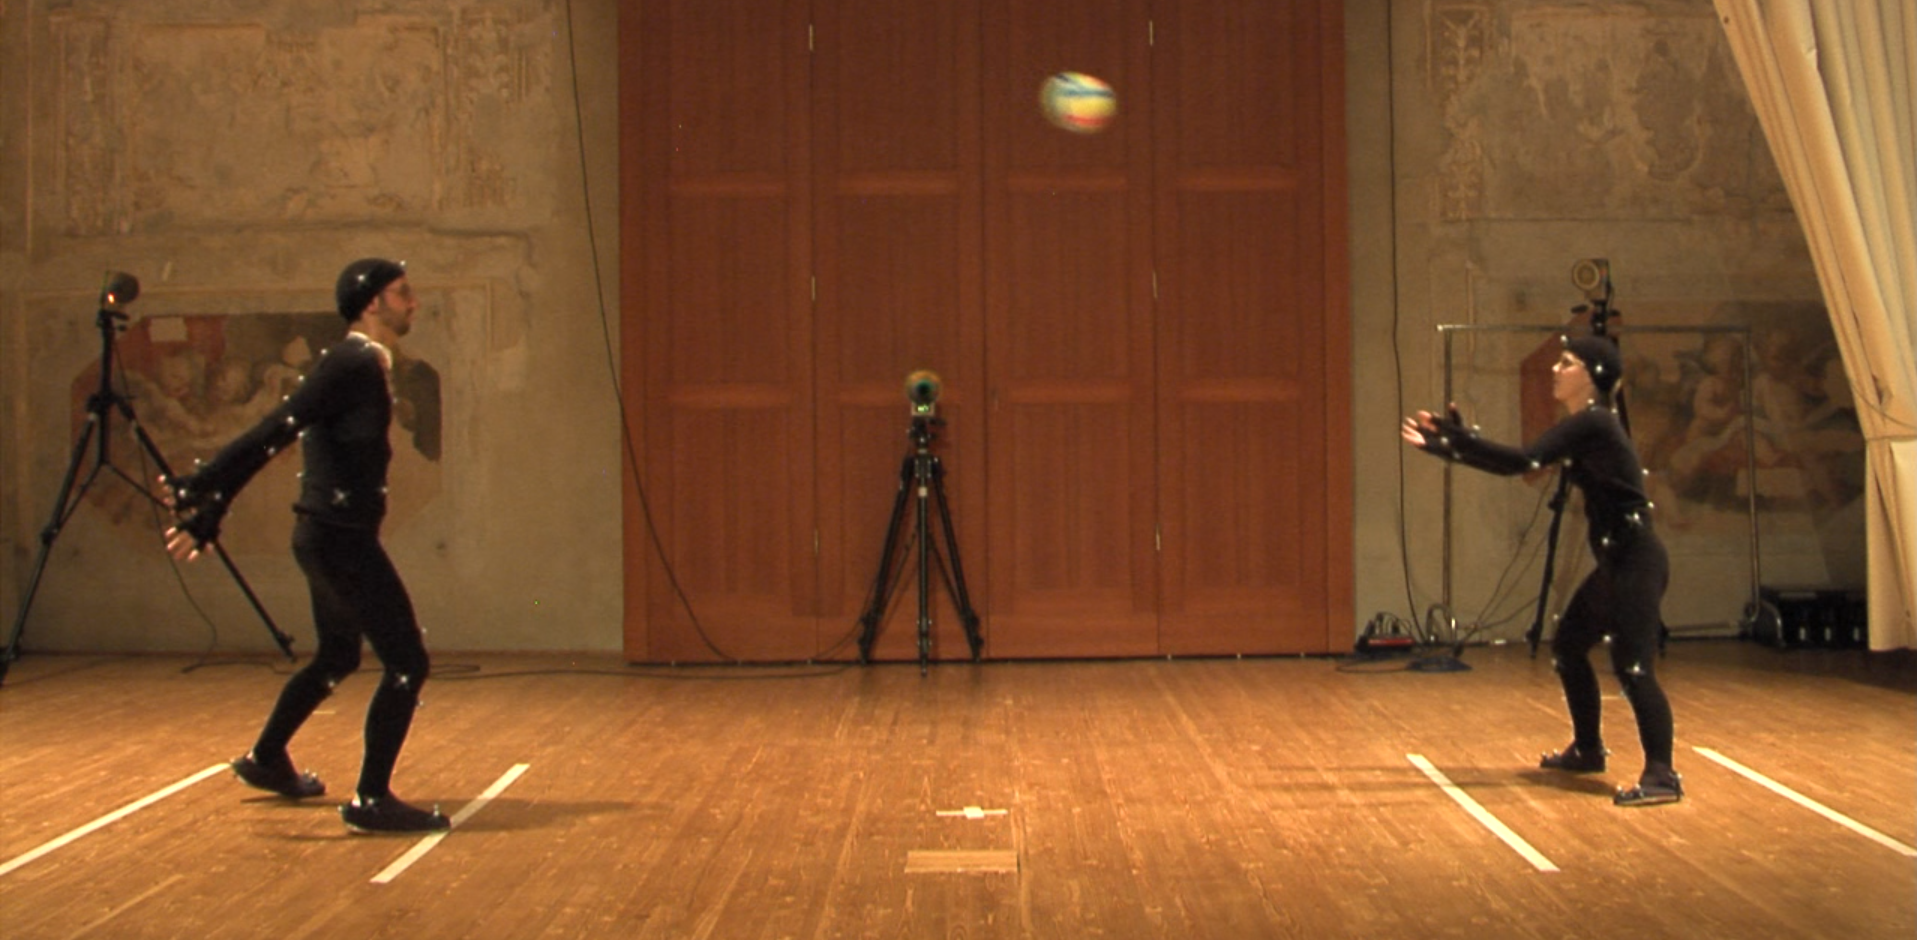
\includegraphics[width=0.75\textwidth]{bodyMarkersExampleImage.png}
    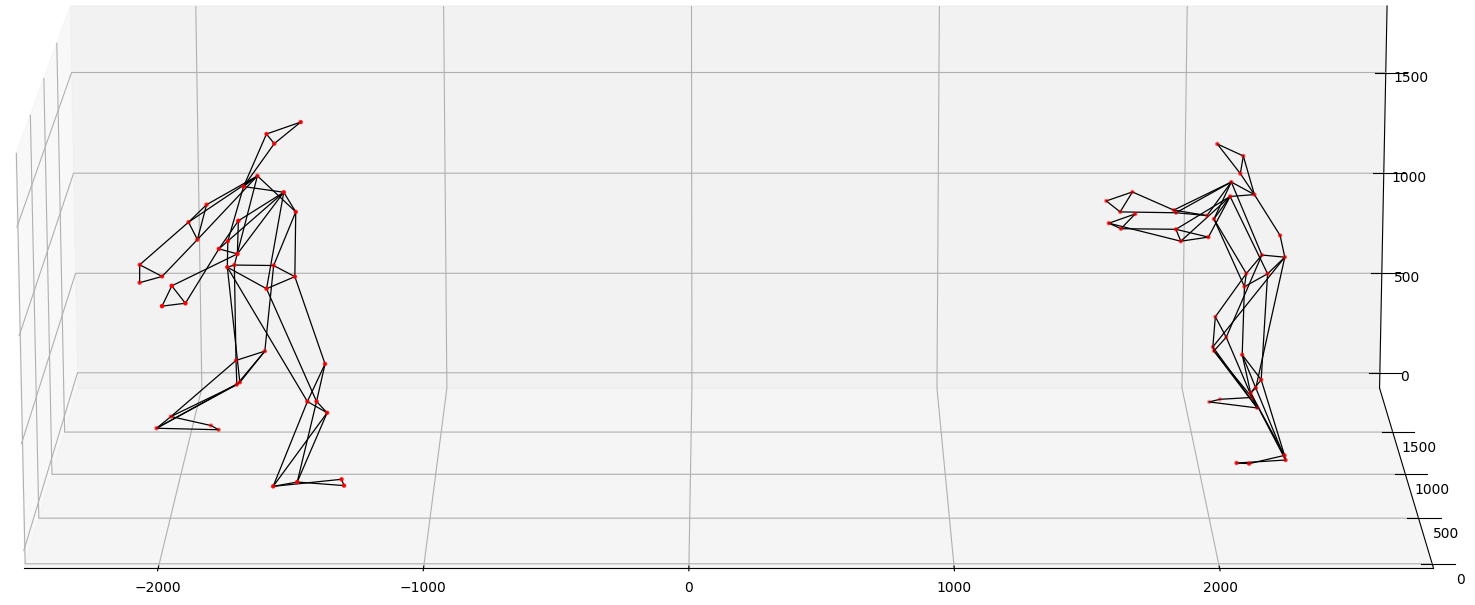
\includegraphics[width=0.75\textwidth]{bodyMarkersExampleMoCap.png}
    \caption{Video frame and MoCap scene with infrared cameras and markers}
    \label{fig:mocap_scene}
\end{figure}
\vspace{-1.5\baselineskip}
However, marker-based MoCap had limitations, including occlusion 
(when markers were hidden from view), inaccuracies, and the need for time-consuming calibration processes. 
These limitations led to the development of markerless MoCap technology. 
Markerless MoCap uses computer vision algorithms to track and reconstruct movement without the need for physical markers. 
This approach relies on complex algorithms that can identify and track features of the human body, 
such as joint positions and skeletal structure, from video footage.


\section{Motivation}
While relationships between emotions and facial expressions or voice changes have been widely explored, 
leading to the availability of feasible methods for real-time automatic analysis, 
full-body movement has not been equally investigated. 
Various studies have shown great potential for inferring about emotions and many other human activities \cite{Bachmann:2020, preiler:2023}. 
Being able to automatically analyse the origin of movement could improve human performances, 
prevent injuries, promote physical activity, develop cognitive and motor rehabilitation strategies \cite{piana:2016}. 

For this reason, the research in human movement has branches in various fields of study such as biomechanics and neuroscience \cite{vaessen:2019}, 
experimental psychology, and theories from the arts and humanities \cite{camurri:2016}. 

The progress made in this field still does not allow a complete and robust classification of the origin of movement, in an automated way, 
because this relies mainly on arbitrary thresholds to distinguish between different origins and current state of the body, 
like if it is moving or standing still. 
For example, to recognize the instant when a movement starts it is required to manually tune 
minimum speed values that are difficult to automate and generalize for every context. 

Furthermore in movement recognition there are a lot of mid-level features, like the joint angles,
or the limb trajectories or the body segment coordination, which can be extracted and exploited by a comprehensive algorithm 
that weights every feature in an optimize manner, resulting in improved accuracy over all the possible approaches 
that work on them individually, because it could take into account the possible interactions and dependencies between them. 
An holistic approach in this way could leverage the complementary informations present in each feature by weighting them 
based on their relative importance. 
One last point to take into consideration is that algorithms based on single features could end up in overfitting the data
while the comprehensive one has more generalization capability. 

This research aims to contribute to the design of accurate and robust systems for the automated analysis of the origin of movement
by exploiting both the current techniques of analysis and the emerging ML approaches, 
which have become feasible thanks to advancements in computational capabilities of modern machines. 
